\begin{exercises} 
  \item A moving particle has its velocity given by the quadratic function $v$ pictured in Figure~\ref{F:5.1.Ez1}.  In addition, it is given that $A_1 = \frac{7}{6}$ and $A_2 = \frac{8}{3}$, as well as that for the corresponding position function $s$, $s(0) = 0.5$.
  \begin{figure}[h]
\begin{center}
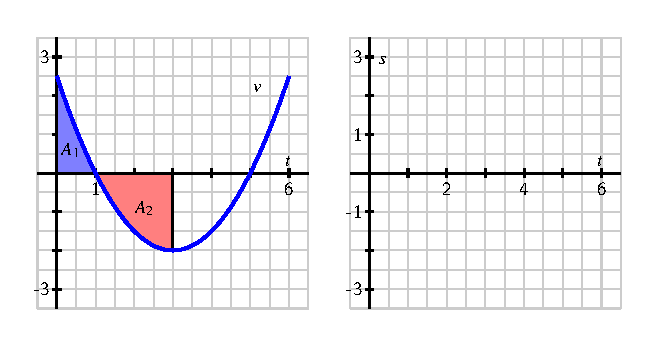
\includegraphics{figures/5_1_Ez1.eps}
\caption{At left, the given graph of $v$.  At right, axes for plotting $s$.} \label{F:5.1.Ez1}
\end{center}
\end{figure}
	\ba
		\item Use the given information to determine $s(1)$, $s(3)$, $s(5)$, and $s(6)$.
		\item On what interval(s) is $s$ increasing?  On what interval(s) is $s$ decreasing?
		\item On what interval(s) is $s$ concave up?  On what interval(s) is $s$ concave down?
		\item Sketch an accurate, labeled graph of $s$ on the axes at right in Figure~\ref{F:5.1.Ez1}.
		\item Note that $v(t) = -2 + \frac{1}{2}(t-3)^2$.  Find a formula for $s$.
	\ea
	
  \item A person exercising on a treadmill experiences different levels of resistance and thus burns calories at different rates, depending on the treadmill's setting.  In a particular workout, the rate at which a person is burning calories is given by the piecewise constant function $c$ pictured in Figure~\ref{F:5.1.Ez2}.  Note that the units on $c$ are ``calories per minute.''
  \begin{figure}[h]
\begin{center}
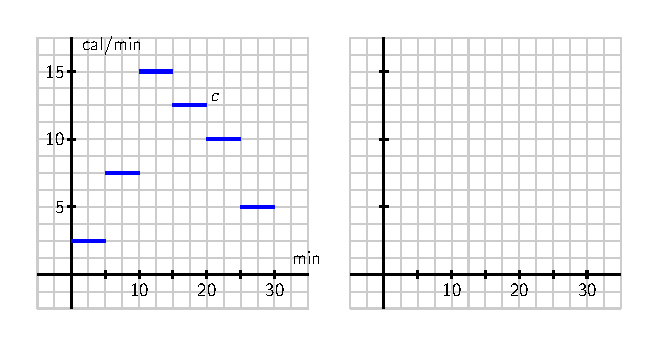
\includegraphics{figures/5_1_Ez2.eps}
\caption{At left, the given graph of $c$.  At right, axes for plotting $C$.} \label{F:5.1.Ez2}
\end{center}
\end{figure}
	\ba
		\item Let $C$ be an antiderivative of $c$.  What does the function $C$ measure?  What are its units?
		\item Assume that $C(0) = 0$.  Determine the exact value of $C(t)$ at the values $t = 5, 10, 15, 20, 25, 30$.
		\item Sketch an accurate graph of $C$ on the axes provided at right in Figure~\ref{F:5.1.Ez2}.  Be certain to label the scale on the vertical axis.
		\item Determine a formula for $C$ that does not involve an integral and is valid for $5 \le t \le 10$.
	\ea

  \item Consider the piecewise linear function $f$ given in Figure~\ref{F:5.1.Ez3}.  Let the functions $A$, $B$, and $C$ be defined by the rules $A(x) = \int_{-1}^{x} f(t) \, dt$, $B(x) = \int_{0}^{x} f(t) \, dt$, and $C(x) = \int_{1}^{x} f(t) \, dt$.
  \begin{figure}[h]
\begin{center}
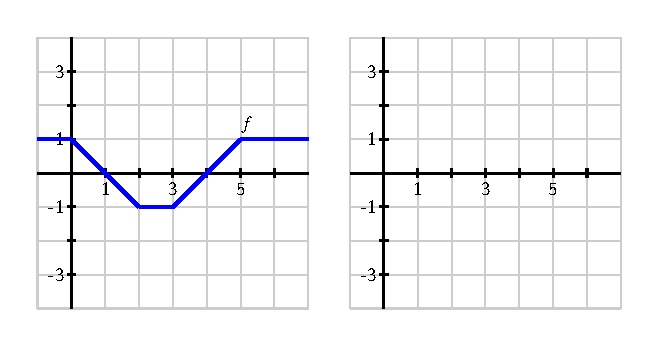
\includegraphics{figures/5_1_Ez3.eps}
\caption{At left, the given graph of $f$.  At right, axes for plotting $A$, $B$, and $C$.} \label{F:5.1.Ez3}
\end{center}
\end{figure}
	\ba
		\item For the values $x = -1, 0, 1, \ldots, 6$, make a table that lists corresponding values of $A(x)$, $B(x)$, and $C(x)$.  
		\item On the axes provided in Figure~\ref{F:5.1.Ez3}, sketch the graphs of $A$, $B$, and $C$.
		\item How are the graphs of $A$, $B$, and $C$ related?
		\item How would you best describe the relationship between the function $A$ and the function $f$?
	\ea



\end{exercises}
\afterexercises


